\documentclass[11pt, a4paper]{article}
\usepackage[utf8]{inputenc}

\usepackage{amsmath,wasysym}
\usepackage{amsrefs}
\usepackage{tikz, wasysym}
\usepackage[]{csquotes}
\usepackage[utf8]{inputenc}
\usepackage[german]{babel}
\usepackage[export]{adjustbox}
\usepackage{pdfpages}

\author{Sven Fiergolla, 1252732}
\title{Portfolio zur Vorlesung Programmierung II}


\begin{document}
 

\clearpage\maketitle
\thispagestyle{empty}
\pagebreak


\section*{Reflexion}

\paragraph*{}
Zu Beginn der Vorlesungsreihe beschäftigten wir uns mit einfachen Datenstrukturen und deren Aufbau, beispielsweise verkettete Listen, binäre Bäume und Schlangen als Wiederholung. Da diese Strukturen als Grundlage für viele der weiterführenden Themen sind, ist die Behandlung dieser notwendig und hilfreich.\\
Ebenso wurde die Funktionsweise von \textit{Interfaces, Streams} und \textit{Exeptionhandling} rekapituliert und den Studenten wurde das \textit{log4j}-Framework zum standardisierten Logging der eigenen Anwendungen erläutert und dessen Verwendung nahegelegt. Mit \textit{Streams} wurde uns die Möglichkeit zur funktionalen Programmierung in Java gegeben, ein Konzept, was im weiteren Verlauf der Vorlesung, durch die Verwendung von Skala, als funktionale Sprache, gefestigt wurde. Anständiges \textit{Exceptionhandling} und \textit{Logging} wurde zwar gelehrt, die wirkliche Bedeutung dieser Konzepte versteht man jedoch erst, wenn man eigene, größere Projekte verfasst, welche ohne jene Konzepte praktisch nicht umzusetzten sind.\\
Anschließend beschäftigren wir uns mit graphischen Benutzeroberflächen unter Gebrauch des GUI-Toolkits \textit{SWING} und erstellten eigene Benutzeroberflächen oder Spiele (Mienenfeger aus der Vorlesung). Auch dies Thema ist von großer Bedeutung, da die meisten Endbenutzeranwendungen nicht auf eine graphische Oberflche verzichten können, um auch von unerfahrenen Anwendern genutzt werden zu können.
\par

\paragraph*{}
In den folgenden Wochen beschäftigten wir uns mit \textit{Nebenläufigkeit} in Form von mehreren Threads in einer Anwendung. Dazu animierten und simmulierten wir mehrere Kugel auf einem Feld, welche miteinander kollidierten. Das Debuggen parallelilsierter Anwendungen stellte sich häufiger als Herrausforderung heraus, da \textit{Deadlocks}und \textit{race conditions} schwierig zu finden sind. Dennoch ist die nebenläufige Prgrammierung vorallem bei rechenintensiven und zeitkritischen Problemen von Nöten.\par


\pagebreak
\section*{Einführung}


\pagebreak
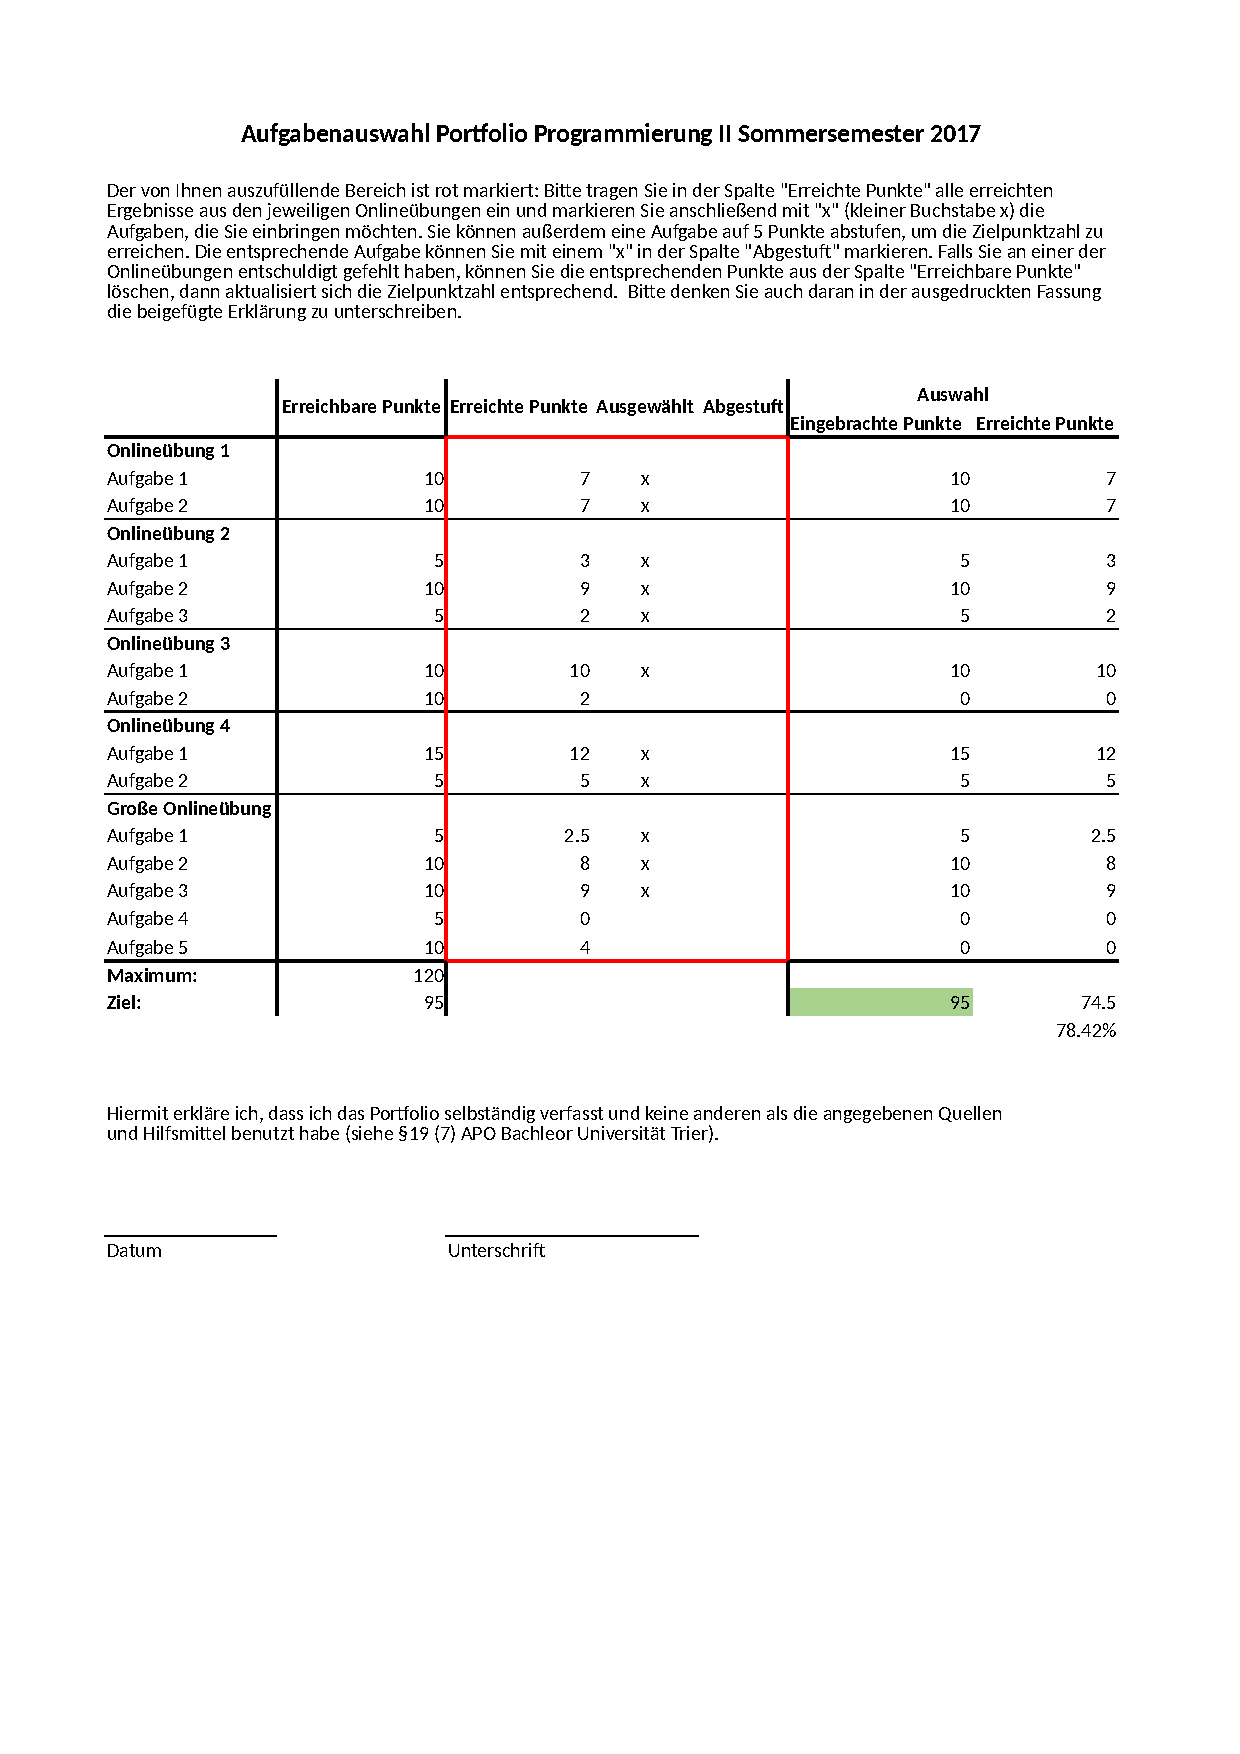
\includepdf[scale=1]{Aufgabenauswahl_Portfolio_FINAL.pdf}



\end{document}